\documentclass{article}
\begin{document}

\subsection{Proizvodi}

Proizvodi predstavljaju slučaj upotrebe u kom se formalizuju usluge koje banka pruža korisnicima. Potrebno je da korisnik podnese zahtev banci za korišćenje određenog proizvoda (lično u banci ili popunjavanjem forme putem online bankarstva). Zahtevi se obrađuju i ako ih banka odobri, korisniku je omoguceno koriscenje proizvoda.

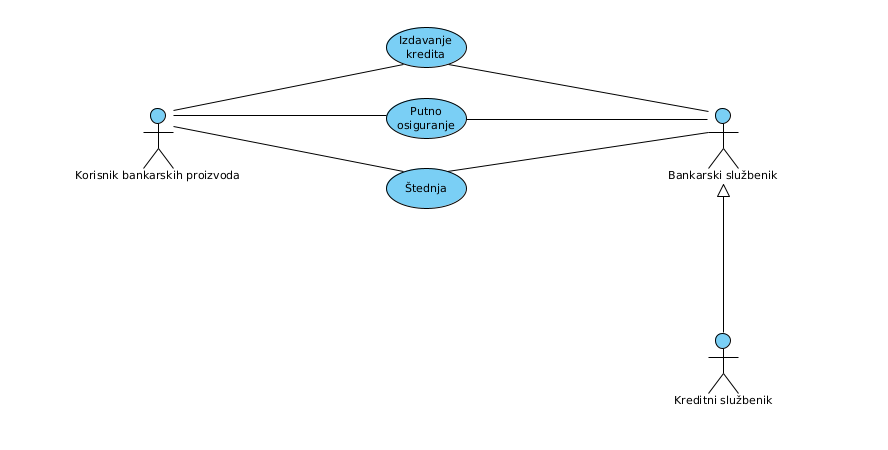
\includegraphics[scale = 0.4]{./UseCases/Pictures/Bank_products.png}

\subsubsection{Slucaj upotrebe: Izdavanje kredita}

Kratki opis: Korisnik šalje zahtev za otvaranje kredita. Banka proverara korisnika, otvara mu račun (ukoliko korisnik već nema otvoren račun u toj banci) i uplaćuje željeni iznos.\\
Učesnici: 
\begin{enumerate}
\item Kreditno odeljenje - kreditni službenik
\item Korisnik proizvda banke
\end{enumerate}
Preduslovi: 
\begin{enumerate}
\item Banka ima u ponudi zahtevani proizvod korisnika
\item Korisnik ima preko 24 godine i u stalnom je radnm odnosu duze od 3 meseca 
\item Zahtev je uspešno dostavljen kreditnom odeljenju za njegovu obradu 
\end{enumerate}
Postuslovi: 
\begin{enumerate}
\item Korisniku je otvoren racun u banci na kom se nalazi zahtevani iznos kredita 
\item Korisniku je uručen plan otplate kredita. 
\end{enumerate}
Glavni tok: 
\begin{enumerate}
\item Korisnik na uvid donosi ličnu kartu 
\item Kreditni službenik (bankar) u sistem unosi zahtev za podizanje kredita 
\item Korisnik od bankara dobija obrazac koji je potrebno da overi u firmi u kojoj je zaposlen 
\item Bankar podatke o firmi unosi u sistem banke 
\item Ovlašćeni radnik banke dobija izveštaj o korisniku od Kreditnog biroa 
\item Kreditno odeljenje banke treba da ustanovi da li je moguce korisniku izdati kredit u željenom iznosu 
\item Ukoliko su svi uslovi ispunjeni, korisnik potpisuje ugovor i menicu 
\end{enumerate}
\end{document}
